% CVPR-style submission source. The fair TEST result slots remain guarded until
% the frozen common-success evaluation and result-dependent writing close.
\documentclass[10pt,twocolumn,letterpaper]{article}
\usepackage[review]{cvpr}
\usepackage{amsmath,amssymb,booktabs,graphicx}
\definecolor{cvprblue}{rgb}{0.21,0.49,0.74}
\usepackage[pagebackref,breaklinks,colorlinks,allcolors=cvprblue]{hyperref}
\def\confName{CVPR}
\def\confYear{2027}
\title{Ray-Based Semantic Evidence Retargeting for Multi-View 3D Editing}
\author{Anonymous authors}
\begin{document}
\maketitle

\begin{abstract}
An edited target image and undeformed source views show different states of
one object. Native multi-view projection can therefore deliver a source
feature to the wrong edited region. We adapt source evidence within a
pretrained pixel-aligned 3D generator while retaining its direct target
conditioning. A frozen semantic matcher proposes source patches, one posterior
is shared by voxels on a camera ray, and a gated source-contrast retargeter
corrects the native carrier. Geometry and appearance stages use separately
selected aggregators. We distinguish candidate retrieval from generated
quality and evaluate geometry, target alignment, source appearance, and image
distribution on source-disjoint edits.
\IfFileExists{final-results/cvpr2027-abstract-findings.tex}{%
\input{final-results/cvpr2027-abstract-findings.tex}
}{%
The common-success held-out comparison is in progress; this source is a
protocol and layout preview, not a submission-ready result report.
}
\end{abstract}

\IfFileExists{final-results/figures/paper-teaser-caption.tex}{%
\begin{figure*}[t]
\centering
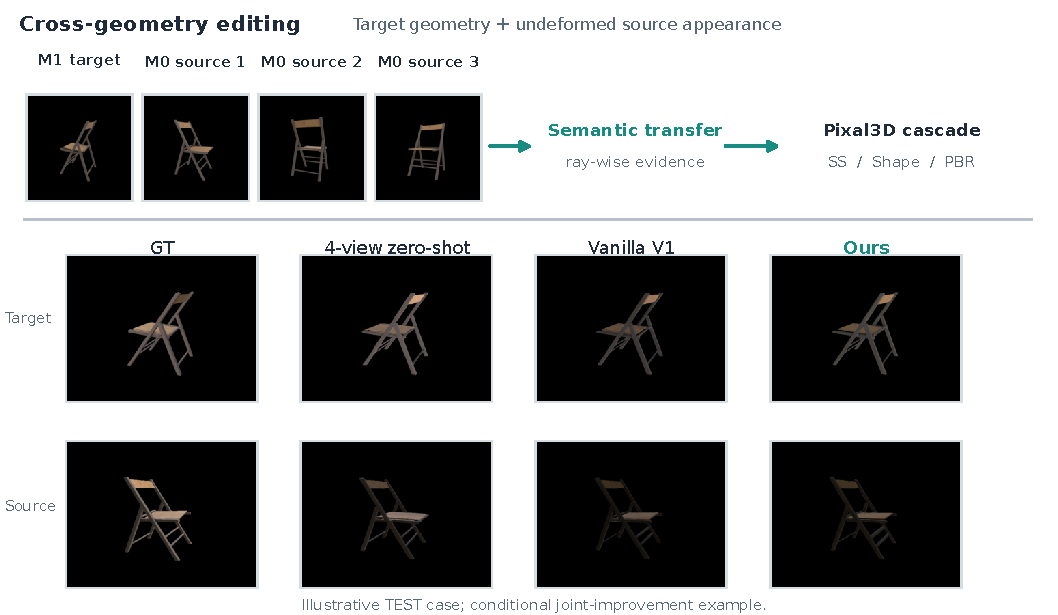
\includegraphics[width=\textwidth]{final-results/figures/paper-teaser.pdf}
\input{final-results/figures/paper-teaser-caption.tex}
\label{fig:cvpr-teaser}
\end{figure*}
}{%
\noindent\textbf{Fair common-success teaser pending.}
}

\section{Introduction}
An image edit can change an object's geometry while its source views retain
the original appearance. These views provide complementary evidence, but
their spatial projections conflict after deformation. The projective carrier
of Pixal3D~\cite{li2026pixal3d} supplies a useful 3D prior; source evidence
must be adapted before it enters that carrier. A single semantic match can
miss the correct region, whereas a broad set can dilute it. Matching quality
alone does not show that the generated shape or material improves.

We study a ray-shared evidence path in the supplied multi-view Pixal3D LoRA
implementation. A frozen VGGT-$\Omega$ matcher~\cite{wang2026vggtomega}
provides proposals and a trained D1 decoder scores them. Distinct observed
target patches associated with one source-camera ray vote into a Top-$K$
posterior. Native source values, rather than a new learned value projection,
are aggregated and fed through a gated retargeter. The edited target retains
its original conditioning route, and unsupported rays retain the native
source path. We select the geometry and appearance stages on their respective
development objectives, then test the frozen composition on held-out edits.

Our contributions are the source-adaptation formulation within a pretrained
projective carrier, matched tests of correspondence and aggregation choices,
and a common-success evaluation that reports target alignment, source
appearance, and registration effects separately. We report uncertainty and
negative results: candidate coverage does not by itself establish a
generated-quality improvement.

\section{Related work}
TRELLIS.2~\cite{xiang2025trellis2} and Pixal3D~\cite{li2026pixal3d}
provide sparse 3D generation and pixel-aligned conditioning. ShapeUP
uses a source mesh with an edited image~\cite{gat2026shapeup}, while
SpaceControl supplies spatial guidance to a pretrained generator
~\cite{fedele2025spacecontrol}. ReconViaGen~\cite{chang2025reconviagen},
MV-Adapter~\cite{huang2025mvadapter}, and CorrAdapter
~\cite{zhang2026corradapter} use different image and correspondence inputs.
Our comparison labels these inputs explicitly. Semantic representations
from VGGT-$\Omega$ and related matching work motivate proposal retrieval,
but the question here is whether those proposals improve a generator when
source and target depict intentionally different shapes.

\section{Method}
\begin{figure*}[t]
\centering
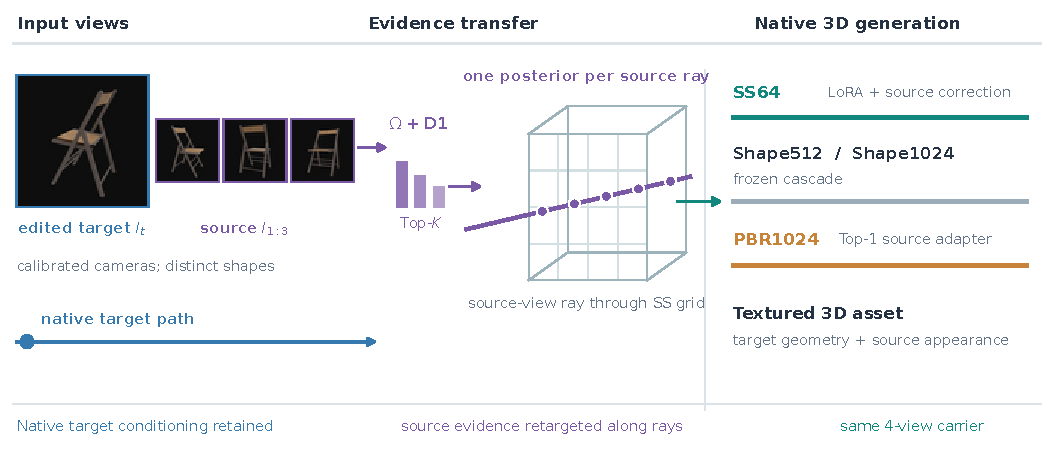
\includegraphics[width=\textwidth]{final-results/figures/paper-overall.pdf}
\caption{The edited target keeps its native conditioning path. Frozen Omega
and D1 produce semantic source proposals; a source-camera ray shares one
posterior, and the gated correction enters SS64. Shape512/1024 stay frozen;
PBR1024 has a separately selected Top-1 source adapter.}
\label{fig:cvpr-overall}
\end{figure*}

\paragraph{Ray-shared proposals.}
Let $C_{\rm MV4}$ be the original four-view carrier and
$\mathcal R_{j,p}=\{x:\pi_j(x)=p\}$ the conditioning-grid sites on source
camera $j$'s image patch $p$. These sites share one evidence decision rather
than learning an independent attention output per voxel. For each observed
target member $m$, D1 scores semantic source proposals $k$. Their
probabilities vote once per member:
\begin{align}
\bar p_r(k)&=|\mathcal M_r|^{-1}\sum_{m\in\mathcal M_r}p_m(k),\\
\mathcal K_r&=\operatorname{Top64}(\bar p_r),\\
p_r(k)&=\frac{\bar p_r(k)}{\sum_{l\in\mathcal K_r}\bar p_r(l)}.
\end{align}
Missing member entries carry zero mass. Training-only topology and depth
define positive proposal IDs for a listwise D1 objective; neither is an
inference input. Omega and D1 are frozen during generative fine-tuning.

\begin{figure}[t]
\centering
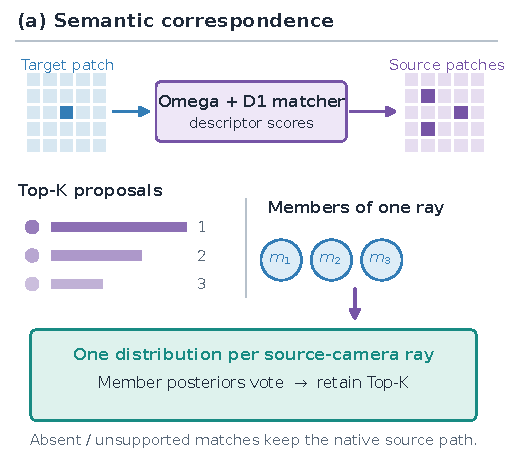
\includegraphics[width=\columnwidth]{final-results/figures/paper-matching.pdf}
\caption{Distinct observed target members vote into a Top-$K$ posterior for
one source-camera ray. Colored patch markers illustrate the mechanism; they
are not measured matches.}
\label{fig:cvpr-matching}
\end{figure}

\paragraph{Evidence delivery.}
The selected SS path uses native DINOv3 values
$E_r=\sum_{k\in\mathcal K_r}p_r(k)v_k$. With source value $S_r$, pooled target
context $T_r$, learned source-use $u_r$, and signed gate $g$, the correction is
\begin{align}
\Delta_r&=u_r\{g(E_r-S_r)+R_\phi([E_r-S_r,T_r])\},\\
C&=C_{\rm MV4}+\tfrac14\sum_{j=1}^{3}P_j(\Delta_j).
\end{align}
The gate and retargeter output start at zero, recovering the pretrained
carrier. Empty-support rays abstain. A confident wrong match is not detected
by this fallback, and target RGB preservation is evaluated rather than
assumed. The appearance stage uses a separate Top-1 retargeter on generated
geometry; Shape512/1024 remain frozen.

\begin{figure}[t]
\centering
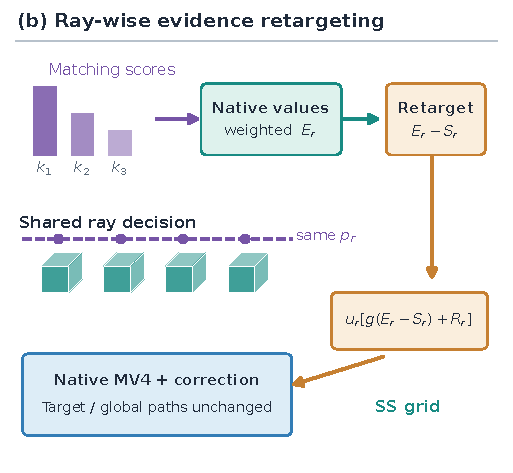
\includegraphics[width=\columnwidth]{final-results/figures/paper-retargeting.pdf}
\caption{Native values are weighted by the ray posterior, contrasted with the
existing source value, and gated into the original carrier. The target path
and unsupported native source path remain available.}
\label{fig:cvpr-retargeting}
\end{figure}

\section{Experiments}
\paragraph{Data and training.}
DeformNeXt-10k contains 10,165 accepted deformations from 3,483 source
assets, split 9,149/508/508 by source asset. Earlier mixed385 multi-view
pretraining is a separate lineage. We continue the supplied complete
base+LoRA multi-view checkpoints, with VGGT-$\Omega$ epoch 7 for matching.
SS64 uses 480 updates and global batch 96; PBR1024 uses 1,900 updates and
batch 24. Both correspond to about five passes. Development SS geometry uses
DEV128 with common frozen downstream stages; PBR appearance uses identical
geometry, guides, noise, and triangles on DEV32. No test example selects
weights, an image-scale estimator, or registration settings.

\paragraph{Fair held-out protocol.}
TEST508 supplies edited target RGB at camera 8, original RGB at cameras
9/10/11, and camera calibration. Our V1 and selected methods use the same
image-only scale estimate, no mesh-derived object scale at generation, and a
1024 cascade. The official Pixal3D RGB1 control receives only target RGB and
its camera; other methods retain their native supported inputs. We report
each native success count and compute rankings on the exact shared success
set. All outputs use a common Cycles/512 render and untouched geometry for
surface scores. Main results apply only post-generation Sim(3) fitted to the
available input source mesh M0; paired raw renders expose its effect. The
edited target M1 is used only for scoring. Source-camera 9/10 metrics are
LPIPS, DreamSim, CLIP, FID, and KID; target-camera 8 metrics are PSNR, SSIM,
and mask IoU. Geometry uses symmetric unsquared Chamfer distance and
F@0.02. Intervals resample source clusters.

\section{Results}
\IfFileExists{final-results/scale-ungiven-main-table.tex}{%
\begin{table*}[t]
\centering\normalsize
\setlength{\tabcolsep}{2.5pt}
\resizebox{\textwidth}{!}{%
\begin{tabular}{llrrrrrrrrrrr}
\toprule
& & & \multicolumn{3}{c}{Source preservation (9/10)} & \multicolumn{2}{c}{Distribution (9/10)} & \multicolumn{5}{c}{Target alignment (8/M1)}\\
Method & Input & Success & LPIPS$\downarrow$ & DreamSim$\downarrow$ & CLIP$\uparrow$ & FID$\downarrow$ & KID$\downarrow$ & PSNR$\uparrow$ & SSIM$\uparrow$ & M-IoU$\uparrow$ & CD$\downarrow$ & F@0.02$\uparrow$\\
\midrule
Ours selected & T1+S3+C & 508/508 & \underline{0.0538} & \underline{0.1352} & \underline{0.9384} & \textbf{38.56} & \underline{0.685} & \textbf{23.28} & \underline{0.9459} & \textbf{0.8619} & \textbf{0.01493} & \textbf{0.8047}\\
Ours vanilla V1 & T1+S3+C & 508/508 & \textbf{0.0536} & \textbf{0.1339} & \textbf{0.9391} & \underline{38.61} & 0.737 & \underline{23.22} & \textbf{0.9463} & \underline{0.8584} & \underline{0.01512} & \underline{0.8032}\\
\midrule
Pixal3D official 1024 (given C) & T1+C & 507/508 & 0.0979 & 0.3629 & 0.8691 & 79.64 & 8.049 & 17.77 & 0.9212 & 0.5302 & 0.05603 & 0.3944\\
\midrule
TRELLIS.2 & T1 & 508/508 & 0.0909 & 0.2539 & 0.9018 & 57.73 & 1.996 & 18.28 & 0.9210 & 0.5633 & 0.05168 & 0.4779\\
Pixal3D official (estimated C) & T1 & 508/508 & 0.0887 & 0.2035 & 0.9211 & 54.06 & 2.806 & 18.77 & 0.9216 & 0.6164 & 0.04419 & 0.4846\\
ReconViaGen & T1+S3 & 508/508 & 0.0731 & 0.1772 & 0.9274 & 45.21 & \textbf{0.637} & 19.88 & 0.9310 & 0.6836 & 0.03607 & 0.5848\\
MVAdapter+ReconViaGen & T1 & 504/508 & 0.0946 & 0.2794 & 0.8933 & 64.65 & 4.169 & 18.26 & 0.9180 & 0.5877 & 0.05236 & 0.4175\\
CorrAdapter+ReconViaGen & T1 & 502/508 & 0.0939 & 0.2767 & 0.8940 & 62.95 & 3.735 & 18.29 & 0.9202 & 0.5835 & 0.05203 & 0.4131\\
ShapeUp & T1+M0 & 508/508 & 0.0853 & 0.2947 & 0.8863 & 72.49 & 6.411 & 18.02 & 0.9218 & 0.6017 & 0.05045 & 0.5170\\
TRELLIS.2+SpaceControl & T1+P+A1 & 508/508 & 0.0913 & 0.2844 & 0.8945 & 62.19 & 2.970 & 17.37 & 0.9179 & 0.5639 & 0.05173 & 0.4726\\
\bottomrule
\end{tabular}}
\caption{Common-success TEST comparison on 501/508 edits. All rows use the same evaluation cameras, Cycles renderer, metric code, and post-generation source-M0-only Sim(3) alignment; no target-derived object scale is supplied at generation. Success is the native method count before the common intersection. T1 is the edited target RGB, S3 three original source RGBs, M0 the textured source mesh, A1 an original anchor RGB, P a TRELLIS.2 target proxy predicted from T1, and C provided camera metadata. Native model input access differs by row; the older Pixal3D baseline estimates C and uses a 1536 cascade, while the new RGB1 and Ours rows use given C and a 1024 cascade. Source metrics use cameras 9/10; target image metrics use camera 8; geometry is measured against edited M1. KID values are multiplied by 1,000 for display. Bold and underline mark the first and second values within this table.}
\label{tab:scale-ungiven-common-main}
\end{table*}

}{%
\noindent\textbf{Frozen common-success ten-method results pending.}
}
\begin{table}[t]
\centering\footnotesize
\setlength{\tabcolsep}{3pt}
\begin{tabular}{lrr}
\toprule
SS development design & CD$\downarrow$ & F@0.02$\uparrow$\\
\midrule
Spatial3, raw cosine & 0.012970 & 0.839333\\
Raw semantic64, cosine & 0.012879 & 0.841031\\
Decoder64, cosine & 0.012807 & 0.842414\\
Decoder64, scalar (Fixed) & 0.012757 & 0.844058\\
Top-1 (No-score) & 0.012780 & 0.840095\\
Uniform on Fixed support & 0.012830 & 0.842505\\
Without retargeter & 0.012956 & 0.835038\\
\bottomrule
\end{tabular}
\caption{Matched DEV128 geometry comparisons with common frozen downstream
stages. Point-estimate trends guide stage selection; adjusted component
intervals include zero. The rows distinguish support, score weighting, and
the physical retargeter rather than treating each as an isolated removal.}
\label{tab:cvpr-ablation}
\end{table}

Raw semantics, decoder descriptors, and scalar scores form a favorable
geometry point-estimate ladder in Table~\ref{tab:cvpr-ablation}. None of the
48 adjusted development component intervals excludes zero. In separate
retrieval diagnostics, exact rank-one coverage rises from 1.25\% to 7.73\%
with D1; member proposal coverage at 64 rises from 50.76\% to 73.36\%.
These are retrieval measurements, not generated-quality claims. Fixed-geometry
PBR DEV32 gives Top-1 retargeting a small LPIPS/DreamSim point advantage,
but its paired intervals include zero.

\IfFileExists{final-results/cvpr2027-results.tex}{%
\input{final-results/cvpr2027-results.tex}
}{%
The fair TEST508 ten-method table, paired V1/selected and official contrasts,
and outcome-conditioned qualitative illustration will be discussed only after
their common-population receipts close.
}

\section{Discussion and limitations}
Source appearance and geometry are measured separately: an SS change can
alter rendered appearance with common PBR, and fixed-geometry PBR comparisons
cannot establish a geometry effect. Candidate coverage need not improve
generation. The final V1-to-selected contrast bundles matching, ray sharing,
and retargeting and cannot assign a causal gain to each component. Camera
metadata and source M0 access differ across native baselines and are labeled
in the comparison. Overlap with earlier multi-view pretraining has not been
audited; input-view metrics do not prove unseen-view quality.

\section{Conclusion}
\IfFileExists{final-results/cvpr2027-conclusion.tex}{%
\input{final-results/cvpr2027-conclusion.tex}
}{%
We formulate semantic evidence retargeting within a pretrained projective
carrier and report matched stage studies. A cross-method conclusion awaits
the frozen, scale-unprovided TEST508 evaluation.
}

\section*{LLM Usage Statement}
An LLM assistant helped with code editing, experiment monitoring, and
manuscript drafting. The authors retain responsibility for validating the
data, analysis, and submitted text.

{\small\bibliographystyle{ieeenat_fullname}\bibliography{references}}
\end{document}
